\documentclass[letterpaper,11pt]{article}
\usepackage{hyperref}
\usepackage{tikz}
\newcommand{\superscript}[1]{\ensuremath{^{\textrm{#1}}}}
\newcommand{\unit}[1]{\ensuremath{\, \mathrm{#1}}}
\newcommand{\inlinecode}{\texttt}

\begin{document}

\title{CS 620: Homework 5}
\date{October 2, 2012}
\author{Carmen St.\ Jean}

\maketitle

\begin{enumerate}
\item \emph{(1.5) If a child dies before its parent calls \emph{wait()}, the child becomes a zombie. What is a zombie (in terms of process data structures)?}

A zombie process is a process that exists only in the process table.
\item \emph{(1.5) What is the reason behind making the child a zombie, instead of just erasing the child completely from memory?}

If a child was simply erased completely from memory, then there would be problems if the child was making usage of system resources.
\item \emph{(3) Unix process management is based on process hierarchy - every process, except init, has a parent. Windows, on the other hand, is not based on hierarchy; all processes are equal. (FYI, when a Windows process is created, the parent is given a token by which it can
control its child, but the parent can pass this token to some other process, thus, invalidating the hierarchy. In Unix, a parent cannot disinherit its children.)}

\begin{enumerate}
\item \emph{Explain one design advantage of the process hierarchy structure.}

One advantage of the process hierarchy structure is that killing a parent also kills its children.  With the process P2P structure, it might be unclear who else should die when a process is killed.
\item \emph{Explain one design advantage of the process P2P (peer-to-peer) structure.}

One advantage of the process P2P structure is that children can exist beyond the life of their parent process.  This might be advantageous if you would like to kill a main process but you would like for some subprocess initiated by it to continue.
\end{enumerate}
\item \emph{(5) For the code below: including the initial parent process, how many processes are created by the above program? Explain and draw the process tree diagram. Write the output in the order in which it is printed.}

\begin{verbatim}
#include <stdio.h>
#include <unistd.h>
int main() {
    /* fork a child process */
    fork(); % a
    wait(&status);
    printf(a) process id = %d, getpid());
    /* fork another child process */
    fork(); % b
    wait(&status);
    printf(b)process id = %d, getpid());
    /* and fork another */
    fork(); % c
    wait (&status);
    printf(c)process id = %d, getpid());
    return 0;
}
\end{verbatim}
Assume that the parent process has the pid of 1 and all subsequent processes are numbered chronologically.  Then the output would be as follows:
\begin{verbatim}
    (a) process id = 2
    (b) process id = 3
    (c) process id = 4
    (c) process id = 3
    (b) process id = 2
    (c) process id = 5
    (c) process id = 2
    (a) process id = 1
    (b) process id = 6
    (c) process id = 7
    (c) process id = 6
    (b) process id = 1
    (c) process id = 8
    (c) process id = 1 
\end{verbatim}
The process tree, using the same pids, would look as pictured below.  The letters a, b, and c represent the three different calls to the fork() method.  These letters have also been added in comments to the code above.

\tikzstyle{level 1}=[level distance=1.25cm, sibling distance=3.25cm]
\tikzstyle{level 2}=[level distance=1.25cm, sibling distance=2.75cm]
\tikzstyle{level 3}=[level distance=1.25cm, sibling distance=2.5cm]
\tikzstyle{level 4}=[level distance=1.5cm, sibling distance=2.25cm]
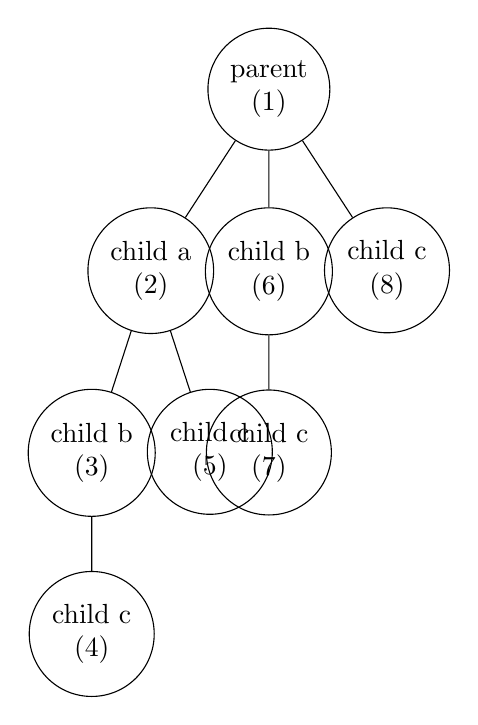
\begin{tikzpicture}
    \tikzstyle{every node}=[circle,draw]
    \node[align=center, below] {parent\\(1)}
        child { 
            node[align=center, below] {child a\\(2)}
            child { node[align=center, below] {child b\\(3)} 
                    child {
                        node[align=center, below] {child c\\(4)} } }
            child { node[align=center, below] {child c\\(5)} } }
        child {
            node[align=center, below] {child b\\(6)}
            child { node[align=center, below] {child c\\(7)} }
        }
        child { node[align=center, below] {child c\\(8)} }
    ;
\end{tikzpicture}
\item \emph{(2.5) Question 3.10: Using the program in Figure 3.29, identify the values of pid at lines A, B, C, and D. (Assume that the actual pids of the parent and child are 2600 and 2603, respectively.) }
\begin{verbatim}
#include <sys/types.h>
#include <stdio.h>
#include <unistd.h>

int main() {
    pid_t pid, pid1;
    
    /* fork a child process */
    pid = fork();
    
    if (pid < 0) { /* error occurred */
        fprintf(stderr, "Fork Failed");
        return 1;
    } else if (pid == 0) { /* child process */
        pid1 = getpid();
        printf("child: pid = %d", pid); /* A */
        printf("child: pid1 = %d", pid1); /* B */
    } else { /* parent process */
        pid1 = getpid();
        printf("parent: pid = %d", pid); /* C */
        printf("parent: pid1 = %d", pid1); /* D */
        wait(NULL);
    }
    
    return 0;
}
\end{verbatim}
The ouput will be:
\begin{verbatim}
child: pid = 0      // A
child: pid1 = 2603  // B
parent: pid = 2603  // C
parent: pid1 = 2600 // D
\end{verbatim}
\item \emph{(2) Question 3.12: Consider the RPC mechanism. Describe the undesirable consequences that could arise from not enforcing either the ``at most once" or ``exactly once" semantic. Describe possible uses for a mechanism that has neither of these guarantees.}

The RPC mechanism is necessary to ensure that a remote process will not be invoked multiple times in a row.  When money is involved, the RPC mechanism is especially critical to prevent multiple processes from being invoked.  Take for example the Cat's Cache cards, which are used to purchase from vending machines and to pay for the washer and driers in dorms.  Students can also load money on to their Cat's Cache card.  The transactions are handled on some remote server.  If this system was not enforcing the ``at most once" mechanism, then a single swipe of the Cat's Cache card could lead to multiple transactions.  This could result in repeat transactions of money being loaded to the card, which would be like producing money out of nowhere.  Or the opposite could happen where the student could be charged multiple times for a single purchase.
\item \emph{(2.5) Suppose there are two processes, P1 and P2, that are on the list of potential programs that could be swapped out (blocked list). Suppose you have to decide which of the 2 processes to swap out. That is, your job is to design the algorithm to determine the victim swap process. What all information (input) do you need to make this selection?}

It would be useful to know the process ID, so that you have a way to refer to each process.  It would also be useful to know what each process is waiting for - e.g., waiting for disk access, waiting for memory access, waiting for network access, etc.  It would be useful to rank the processes in terms of which one would be waiting the longest - e.g., a process waiting for the disk will be waiting longer than a process waiting for memory so it might be a better candidate for being swapped out.  The size of what its waiting for is also very important to know - e.g., it might be better to swap out a process waiting for large amounts of memory than a process waiting to write a small amount of memory from the disk.
\item \emph{(4) Process creation has been divided into two stages - the \emph{fork()} which creates a clone (child) process, and the \emph{execvp()} that makes the forked child different from its parent. The designers could have chosen to develop a single procedure to perform both creation and separation. Give 3 advantages of the \emph{fork()}-\emph{exec()} design over the single procedure design.}

One advantage is that you have two processes - parent and child - that are clearly aware of each other.  Another advantage is that fork can fail, so having two stages to the fork procedure helps you to see which part specifically failed.  A third advantage is that it is easier to police two processes should one of them have a problem.
\item \emph{(3) This question relates to Chapter 1 and the memory hierarchy model:}

\emph{Consider a cache-memory-disk-cloud hierarchy: $cat = 10\unit{ ns}$, $mat = 200\unit{ ns}$; $dat = 10\unit{ ms}$; $clat = 200\unit{ ms}$ ($clat$ = CLoud access time). Suppose the average data access time is $1.6\unit{ ms}$. It is given that $h_c = 60\%$, $h_d = 95\%$ ($h_c = \unit{cache\ hit\ rate}$, $h_d = \unit{disk\ hit\ rate}$). What is the memory hit rate ($h_m$)?}

The formula for average access time, $t$, is given by:
$$
t = h_c\cdot cat + (1 - h_c)[h_m\cdot(cat + mat) + (1 - h_m)[h_d\cdot(cat + mat + dat) + (1 - h_d)\cdot(cat + mat + dat + clat)]]
$$

Since 10 ms = $10^6$ ns, $dat = 10^7$ ns, $clat = 2\cdot10^8$ ns, and average access time is $1.6\cdot10^6$ ns, then:
\begin{eqnarray*}
1600000 &=& h_c\cdot 10 + (1 - h_c)[h_m\cdot210 + (1 - h_m)[h_d\cdot10000210 + (1 - h_d)\cdot210000210]] \\
1600000 &=& 0.60\cdot 10 + 0.4\cdot[h_m\cdot210 + (1 - h_m)[0.95\cdot10000210 + 0.05\cdot210000210]] \\
1600000 &=& 6 + 0.4\cdot[h_m\cdot210 + (1 - h_m)[9500199.5 + 10500010.5]]  \\
1599994 &=& 0.4\cdot[h_m\cdot210 + (1 - h_m)[20000210]] \\
3999985 &=& h_m\cdot210 + (1 - h_m)[20000210] \\
3999985 &=& 210 h_m + 20000210 - 20000210 h_m \\
-16000225 &=& -20000000 h_m \\
h_m &=& 0.80
\end{eqnarray*}
Thus, the memory hit rate is 80\%.
\end{enumerate}

\end{document}